

\begin{frame}[plain,c]
\begin{center}
{\Huge \bf Optional reading for Lecture \thislecture}
\end{center}
\end{frame}


%
%
%

\begin{frame}{Physical origin of diamagnetism}

Consider an electron orbiting a nucleus:\\
\vspace{0.3cm}

\begin{columns}
  \begin{column}{0.35\textwidth}
    \begin{center}
      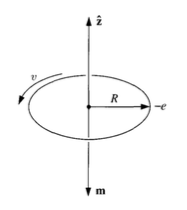
\includegraphics[width=0.94\textwidth]{./images/schematics/orbiting_electron_magnetic_dipole_moment.png}\\
    \end{center}
  \end{column}
  \begin{column}{0.65\textwidth}
     For time intervals much larger than the period of rotation T,
     we may think of the orbiting electron as a {\em steady} current I:
     \begin{equation*}
        I = \frac{q}{T} = - \frac{eu}{2\pi R}
     \end{equation*}
     where u is the electron velocity and R is the radius of its orbit (taken to be circular).
  \end{column}
\end{columns}

\vspace{0.4cm}

The {\bf magnetic dipole moment associated with that orbital motion} is:
\begin{equation*}
  \vec{m} = I \vec{S} = \Big( - \frac{eu}{2\pi R} \Big) \Big( \pi R^2 \hat{z} \Big) \Rightarrow
  \vec{m} = - \frac{1}{2} e u R \hat{z}
\end{equation*}

\end{frame}

%
%
%

\begin{frame}{Physical origin of diamagnetism}

Within an external $\vec{B}$ field, there is a significant effect on the electron orbit.

\begin{columns}
  \begin{column}{0.25\textwidth}
    \begin{center}
      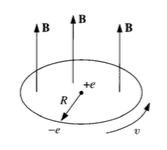
\includegraphics[width=0.90\textwidth]{./images/schematics/orbiting_electron_in_magnetic_field.png}\\
    \end{center}
  \end{column}
  \begin{column}{0.75\textwidth}
     In the absence of a $\vec{B}$ field, Coulomb's force (due to the nucleus) provides centripetal acceleration:
     \begin{equation*}
        \frac{1}{4\pi \epsilon_0} \frac{e^2}{R^2} = m_e \frac{u^2}{R}
     \end{equation*}
  \end{column}
\end{columns}
In the presence of a $\vec{B}$ field, there is an additional force $-e \Big( \vec{u} \times \vec{B} \Big)$.

Assuming (for simplicity) that $\vec{B}$ is perpendicular to the orbital plane, then:
\begin{equation*}
   \frac{1}{4\pi \epsilon_0} \frac{e^2}{R^2} + e \bar{u} B = m_e \frac{\bar{u}^2}{R} \Rightarrow
   m_e \frac{u^2}{R} + e \bar{u} B = m_e \frac{\bar{u}^2}{R} \Rightarrow
\end{equation*}
\begin{equation*}
    e \bar{u} B = \frac{m_e}{R} \Big( \bar{u}^2 - u^2 \Big) \Rightarrow
    e \bar{u} B = \frac{m_e}{R} \Big( \bar{u} + u \Big)  \Big( \bar{u} - u \Big)
\end{equation*}

\end{frame}


%
%
%

\begin{frame}{Physical origin of diamagnetism}

Assuming that the change ${\Delta}u = \bar{u} - u$ is small, so that $\bar{u} + u \approx 2u \approx 2\bar{u}$,
we can write the previous equation as:
\begin{equation*}
    e \bar{u} B = \frac{m_e}{R} \Big( \bar{u} + u \Big)  \Big( \bar{u} - u \Big) \Rightarrow
    e \cancel{\bar{u}} B = \frac{m_e}{R} 2 \cancel{\bar{u}} {\Delta}u \Rightarrow
\end{equation*}
\begin{equation*}
    {\Delta}u = \frac{eRB}{2m_e}
\end{equation*}
In the presence of a $\vec{B}$ field, the electron velocity increases by ${\Delta}u$.
This changes its magnetic dipole moment:
\begin{equation*}
  \vec{m} = - \frac{1}{2} e u R \hat{z}
\end{equation*}
The change $ {\Delta}\vec{m}$ is given by:
\begin{equation*}
    {\Delta}\vec{m} =
      - \frac{1}{2} e {\Delta}u R \hat{z} =
      - \frac{1}{2} e \Big( \frac{eRB}{2m_e} \Big) R \hat{z} \Rightarrow
    {\Delta}\vec{m} =
      - \frac{e^2 R^2}{4m_e} \vec{B}
\end{equation*}

\end{frame}

% ------------------------------------------------------------------------------

%
% Worked example :
%

{
\problemslide

%
%
%

\begin{frame}{Worked example: Free current on circular wire}

  \begin{blockexmplque}{Question}
    An infinite straight wire with a circular cross-section
    of radius $R$ is lying along the $z$ axis
    and it has an internal $\vec{H}$ field given by
    \begin{equation*}
      \vec{H} = \frac{J_0}{r} \Big(\frac{1}{a^2} sin(ar) - \frac{r}{a} cos(ar) \Big) \hat{\phi}
    \end{equation*}
    where
    $r$ is the radial distance from the centre of the circular conductor,
    $\hat{\phi}$ is the azimuthal unit vector,
    $J_0$ is a constant current density,
    and $a$=$\pi/(2R)$.
    Find an expression for the total free current in the conductor,
    and give its direction.
  \end{blockexmplque}

  The free current $I$ can be computed from Ampere's law:
  \begin{equation*}
    I = \oint_{L} \vec{H} \cdot d\vec{\ell}
  \end{equation*}

\end{frame}

%
%
%

\begin{frame}{Worked example: Free current on circular wire}

  Using the given $\vec{H}$ field, and using $a=\pi/2R$, as given,
  the previous expression for $I$ becomes:
  \begin{equation*}
    I = \oint_{L} \frac{J_0}{r}
     \Big(\frac{2R}{\pi^2} sin(\frac{\pi r}{2R}) - \frac{2Rr}{\pi} cos(\frac{\pi r}{2R}) \Big) \hat{\phi}
     \cdot d\vec{\ell}
  \end{equation*}

  To calculate the total free current in the circular conductor, we choose
  a closed circular path with radius equal to the radius of the conductor.
  The element $d\vec{\ell}$ can be written as:
  \begin{equation*}
     d\vec{\ell} = R d\phi \; \hat{\phi}
  \end{equation*}

  Using the above expression for $d\vec{\ell}$, and substituting $r = R$,
  into the our last expression for $I$, we find:
  \begin{equation*}
    I = \int_{0}^{2\pi} \frac{10^4}{R}
     \Big(\frac{4R^2}{\pi^2} sin(\frac{\pi R}{2R}) - \frac{2R^2}{\pi} cos(\frac{\pi R}{2R}) \Big) \hat{\phi}
      \cdot \Big( R d\phi \; \hat{\phi} \Big) \xRightarrow{\hat{\phi} \cdot \hat{\phi} = 1}
  \end{equation*}

\end{frame}

%
%
%

\begin{frame}{Worked example: Free current on circular wire}

  \begin{equation*}
    I = \frac{J_0}{R}
     \Big(\frac{4R^2}{\pi^2} \cancelto{1}{sin(\frac{\pi}{2})} - \frac{2R^2}{\pi} \cancelto{0}{cos(\frac{\pi}{2})} \Big)
      R \int_{0}^{2\pi} d\phi \Rightarrow
  \end{equation*}

  \begin{equation*}
    I = \frac{J_0}{\cancel{R}} \frac{4R^2}{\pi^{\cancel{2}}} \cancel{R} 2\cancel{\pi} \Rightarrow
  \end{equation*}

  \begin{equation*}
    I = \frac{8 J_0}{\pi} R^2
  \end{equation*}

  Since $\vec{H}$ is an azimuthal vector,
  the free current flows in the positive $z$ axis.

\end{frame}

} % Worked example

% ------------------------------------------------------------------------------
% ------------------------------------------------------------------------------

%
% Worked example :
%

{
\problemslide

%
%
%

\begin{frame}{Worked example: Toroid with square iron core}

  \begin{blockexmplque}{Question}
    \begin{minipage}[r]{0.82\textwidth}
      A toroid having an iron core of square cross-section and permeability $\mu$
      is wound with $N$ closely spaced turns of wire carrying a current $I$.
      Find an expression for the magnitude of the magnetisation $M$ everywhere
      inside the iron core.
    \end{minipage}
    \begin{minipage}[l]{0.15\textwidth}
     \begin{center}
       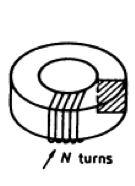
\includegraphics[width=0.94\textwidth]{./images/problems/lect07_toroid_with_square_iron_core}
     \end{center}
    \end{minipage}
  \end{blockexmplque}

  The magnetisation $M$ inside the iron core is:
  \begin{equation*}
    M = \frac{B}{\mu_0} - H
  \end{equation*}

  According to Ampere's circuital law:
  \begin{equation*}
    \oint_{L} \vec{H} \cdot d\vec{\ell} = I_{free} = N I
  \end{equation*}
  where $I_{free}$ is the free current through an open area $S(L)$
  whose boundary is the closed path $L$, and $I$ is the current on
  each of the $N$ windings.

\end{frame}

%
%
%

\begin{frame}{Worked example: Toroid with square iron core}

  Considering the cylindrical symmetry of the problem, $\vec{H}$ is azimuthal.
  Therefore, for a closed path $L$ which is concentric to the iron core,
  perpendicular to the symmetry axis of the toroid,
  and lies within the core:
  \begin{equation*}
    \oint_{L} \vec{H} \cdot d\vec{\ell} = H 2\pi r
  \end{equation*}

  Therefore, Ampere's circuital law yields:
  \begin{equation*}
    H 2\pi r = N I \Rightarrow H = \frac{NI}{2\pi r}
  \end{equation*}

  The magnetic field $B$ can be computed from $H$ as follows:
  \begin{equation*}
     B = \mu H
  \end{equation*}

  Substituting the above into our initial expession for $M$, we find:
  \begin{equation*}
    M = \frac{\mu H}{\mu_0} - H
      = \Big( \frac{\mu}{\mu_0} - 1 \Big) H
      = \Big( \frac{\mu}{\mu_0} - 1 \Big) \frac{NI}{2\pi r}
  \end{equation*}

\end{frame}

} % Worked example
